\documentclass{tudelft-report}



%% Set up the bibliography
\usepackage[backend=biber,style=numeric]{biblatex}
\addbibresource{report.bib}
% \usepackage[backend=biber]{biblatex}
% \addbibresource{report.bib}
\usepackage[colorinlistoftodos]{todonotes}
\usepackage{amsmath,amssymb}
\usepackage{algorithm}
\usepackage{algpseudocode}
\usepackage{float}
%% Additional packages and commands
\setlist{itemsep=-2pt} % Reducing white space in lists slightly
\renewcommand{\deg}{\si{\degree}\xspace} % Use \deg easily, everywhere

%% ----------------------------------------------------------------------
%%    Begin of document + Frontmatter (Roman page numbering)
%% ----------------------------------------------------------------------

\usepackage{tgadventor}
\usepackage{amsmath}
\usepackage{breqn}
\usepackage{longtable}
\usepackage{booktabs}
\usepackage{multirow}
\usepackage{tabularx}
\usepackage{booktabs}
\usepackage{tikz}
\usepackage{graphicx}

% Nomenclature package
\usepackage[intoc]{nomencl}
\makenomenclature

% Optional: group titles (Abbreviations / Symbols)
\renewcommand{\nomgroup}[1]{%
\ifthenelse{\equal{#1}{A}}{\item[\textbf{Abbreviations}]}{%
\ifthenelse{\equal{#1}{S}}{\item[\textbf{Symbols}]}{}}}
\usepackage{ifthen}
\usepackage{graphicx}
\usepackage{tikz}
\usepackage{eso-pic} % <-- important

% --- icons for qualitative tables ---
\usepackage{amssymb}

\newcommand{\High}{\checkmark}   % High  (✓)
\newcommand{\Med}{$\sim$}        % Medium (single curly bar)
\newcommand{\Low}{$\times$}      % Low (×)



\begin{document}

\renewcommand{\figureautorefname}{Figure}
\renewcommand{\tableautorefname}{Table}
\renewcommand{\partautorefname}{Part}
\renewcommand{\appendixautorefname}{Appendix}
\renewcommand{\chapterautorefname}{Chapter}
\renewcommand{\sectionautorefname}{Section}
\renewcommand{\subsectionautorefname}{Section}
\renewcommand{\subsubsectionautorefname}{Section}

\frontmatter

% %% Define the main parameters
% \title{Communication-Enhanced MAPPO for Coordinated ACP Teams in Strike–EA Missions}
% \subtitle{Master Thesis AE}


% \subject{} % Cover only
% \affiliation{Delft University of Technology} % Cover only
% \coverimage{/figures/TMA_bio_plot.png} % Aspect ratio of 2:3 (portrait) recommended
% % \includegraphics[width=0.6\textwidth]{figures/TMA_bio_plot.png}\par\vspace{1cm}
% \definecolor{title}{HTML}{4884d6} % Color for cover title

% \makecover

%% Define the main parameters
\title{Communication-Enhanced MAPPO for Coordinated ACP Teams in Strike-EA Missions}
\subtitle{Mid-Term Report}
\author{Cem Celikbas}
\date{\today} % or a fixed date

\subject{} % Cover only
% \affiliation{Delft University of Technology} % Cover only
\coverimage{figures/cover.png} % usually no leading slash
\definecolor{title}{HTML}{FFFFFF}
% Put logo on the cover page (foreground)
\AddToShipoutPictureFG*{%
  \begin{tikzpicture}[remember picture,overlay]
    \node[anchor=south,yshift=8mm] at (current page.south) {%
      
\includegraphics[width=4cm]{figures/TU_P5_white.png}%
    };
  \end{tikzpicture}%
}
\makecover


\input{frontmatter/title-thesis}
%\chapter*{Preface}
\addcontentsline{toc}{chapter}{Preface}



\begin{flushright}
{\makeatletter\itshape
    \@author \\
    Delft, \monthname{} \the\year{}
\makeatother}
\end{flushright}

%\input{frontmatter/summary}

\setcounter{tocdepth}{1}
\tableofcontents
% \listoffigures
% \listoftables
\chapter*{Nomenclature}
% \addcontentsline{toc}{chapter}{Nomenclature}

%==================================================
% Abbreviations
%==================================================
\section*{Abbreviations}

\begin{description}

% FULL abbreviation list found in the document (cleaned + de-duplicated)

\item[2D] Two-dimensional
\item[3D] Three-dimensional

\item[ABM] Agent-Based Modeling
\item[ACO] Ant Colony Optimization
\item[ACP] Autonomous Collaborative Platform(s)
\item[AFB] Air Force Base
\item[AI] Artificial Intelligence
\item[BT] Behavior Tree
\item[BVR] Beyond-Visual-Range

\item[C2] Command and Control
\item[CA] Cooperative Attacking
\item[CCA] Collaborative Combat Aircraft
\item[CLCE] Centralized Learning with Centralized Execution
\item[CNN] Convolutional Neural Network
\item[CNP] Contract Net Protocol
\item[Comm-MAPPO] Communication-Enhanced MAPPO
\item[CTDE] Centralized Training and Decentralized Execution

\item[DDPG] Deep Deterministic Policy Gradient
\item[DEAD] Destruction of Enemy Air Defenses
\item[DMPC] Distributed Model Predictive Control
\item[DQN] Deep Q-Network
\item[DTDE] Decentralized Training with Decentralized Execution

\item[EA] Electronic Attack
\item[ECM] Electronic Countermeasures
\item[ECNP] Extended Contract Net Protocol
\item[EJ] Escort Jammer(s)
\item[EM] Electromagnetic
\item[EO] Electro-Optical
\item[EW] Electronic Warfare

\item[FEBA] Forward Edge of the Battle Area
\item[FL] Federated Learning
\item[FMARL] Federated Multi-Agent Reinforcement Learning
\item[FOFE] Flexible Observation Feature Encoding

\item[GA] Genetic Algorithm
\item[GAE] Generalized Advantage Estimation
\item[GNSS] Global Navigation Satellite System
\item[GPS] Global Positioning System

\item[HF] High-Fidelity
\item[HMARL] Hierarchical Multi-Agent Reinforcement Learning
\item[HRL] Hierarchical Reinforcement Learning

\item[IADS] Integrated Air Defense System
\item[IAPPO] Independent Asynchronous Proximal Policy Optimization
\item[IMU] Inertial Measurement Unit
\item[INS] Inertial Navigation System
\item[IPPO] Independent Proximal Policy Optimization
\item[ISR] Intelligence, Surveillance, and Reconnaissance

\item[JSR] Jamming-to-Signal Ratio

\item[MADDPG] Multi-Agent Deep Deterministic Policy Gradient
\item[MADQN] Multi-Agent Deep Q-Network
\item[MAFRL] Multi-Agent Federated Reinforcement Learning
\item[MAPPO] Multi-Agent Proximal Policy Optimization
\item[MARL] Multi-Agent Reinforcement Learning
\item[MCAV] Mission Control Aerial Vehicle
\item[MDP] Markov Decision Process
\item[MILP] Mixed-Integer Linear Programming
\item[MPC] Model Predictive Control
\item[MPP] Mission Planning Problem
\item[MTSP] Multiple Traveling Salesman Problem

\item[NFZ] No-Fly Zone
\item[NN] Neural Network

\item[OODA] Observe–Orient–Decide–Act

\item[POMDP] Partially Observable Markov Decision Process
\item[PhD] Doctor of Philosophy
\item[PPO] Proximal Policy Optimization
\item[PSD] Power Spectral Density
\item[PSO] Particle Swarm Optimization

\item[QMIX] QMIX (Q-value mixing network method)
\item[RF] Radio Frequency
\item[RL] Reinforcement Learning
\item[RNN] Recurrent Neural Network
\item[RRT] Rapidly-exploring Random Tree

\item[SA] Situation Awareness
\item[SAM] Surface-to-Air Missile
\item[SEAD] Suppression of Enemy Air Defenses
\item[SNR] Signal-to-Noise Ratio
\item[SOJ] Stand-Off Jamming
\item[SPJ] Self-Protection Jamming

\item[TA] Target Allocation
\item[TD] Temporal Difference

\item[UAV] Unmanned Aerial Vehicle
\item[UCAV] Unmanned Combat Aerial Vehicle
\item[UxV] Unmanned Vehicle (generic)

\end{description}

%==================================================
% Symbols
%==================================================
\section*{Symbols}

\begin{description}

% Radar / EW
\item[$P_t$] Radar transmitted power
\item[$P_r$] Received radar power
\item[$P_j$] Jammer transmitted power
\item[$P_{j,r}$] Jamming power received at the radar  % MISSING
\item[$G_t$] Radar transmit antenna gain
\item[$G_r$] Radar receive antenna gain
\item[$G_j$] Jammer antenna gain
\item[$\lambda$] Signal wavelength
\item[$\sigma$] Radar cross section (RCS)
\item[$R$] Range or distance
\item[$R_{jr}$] Jammer–radar distance  % MISSING
\item[$k$] Boltzmann constant  % MISSING
\item[$T_s$] System noise temperature  % MISSING
\item[$N$] Noise power
\item[$B_n$] Receiver bandwidth
\item[$L$] System losses
\item[$\mathrm{SNR}$] Signal-to-noise ratio
\item[$\mathrm{JSR}$] Jamming-to-signal ratio
\item[$R_{BT}$] Burn-through range

% UAV Kinematics
\item[$(x_i,y_i)$] Position of UAV $i$
\item[$v_i$] Speed of UAV $i$
\item[$\psi_i$] Heading angle
\item[$\omega_i$] Yaw rate

% Reinforcement Learning
\item[$s_i$] State or observation of agent $i$
\item[$a_i$] Action of agent $i$
\item[$r_i$] Reward of agent $i$
\item[$\gamma$] Discount factor
\item[$\theta$] Policy parameters
\item[$\epsilon$] PPO clipping parameter
\item[$\hat{A}$] Advantage estimate
\item[$V(s)$] Value function
\item[$\alpha$] Learning rate
\item[$\tau$] Target network update rate
\item[$K$] Mini-batch size
\item[$t$] Time step

\end{description}

%% ----------------------------------------------------------------------
%%    Mainmatter (Arabic page numbering)
%% ----------------------------------------------------------------------

\mainmatter

\chapter{Introduction}


\section{Related Works}


\section{Foundational Algorithm: PPO}



\chapter{Methodology}

This chapter outlines the methodology used in this thesis. First XXXXX. 

\section{Problem Formulation}

The cooperative striker–jammer engagement is modelled as a
Dec-POMDP $\langle \mathcal{N}, \mathcal{S}, \{\mathcal{A}_i\},
\{\mathcal{O}_i\}, P, \mathcal{R}, \gamma\rangle$ in a two-dimensional
plane. The agent set $\mathcal{N} = \mathcal{N}_s \cup \mathcal{N}_j$
is partitioned into $N_s$ \emph{strikers} and $N_j$ \emph{jammers},
operating in an environment containing a set of radars $\mathcal{R}$
and a set of protected targets $\mathcal{T}$. The team objective is to
destroy all targets in $\mathcal{T}$; jammers degrade adversary radar
coverage to clear penetration corridors for the strikers. 

\subsection{Agents}

Each agent $i$ has continuous state $s_i = [x_i, y_i, v_i, \psi_i,
\dot{\psi}_i]^{\top}$ and follows unicycle kinematics with
piecewise-constant acceleration commands.

\subsubsection{Observation Space}
Agents are partially observed. Each agent has a sensing radius
$R_{\text{obs}}$ inside which it directly detects other agents,
radars, and targets. The local observation
$o_i \in \mathcal{O}_i$ is decomposed into four entity-typed channels:
a fixed-size ego vector
$o_i^{\text{self}} = (x_i, y_i, v_i, \psi_i, \dot{\psi}_i, \tau)$
with $\tau$ the normalised episode time, and three variable-length
sets containing relative bearing, range, and entity-specific features
for visible teammates, radars, and targets, respectively.\footnote{
Per-entity feature dimensions are
$d_{\text{agent}}=4$, $d_{\text{radar}}=3$, $d_{\text{target}}=3$;
masked entries are zeroed.}

\subsubsection{Communication}
Agents share observations over a range-limited, multi-hop graph
following \cite{Wang2025CooperativeUAV}. The set of agents in
\emph{direct} communication with $i$ is
\begin{equation}
\mathcal{N}_i^{1} = \bigl\{ i' \in \mathcal{N} \setminus \{i\}
\;\bigl|\; \rho_{ii'} \le R_{\text{comm}} \bigr\},
\label{eq:comm_direct}
\end{equation}
where $\rho_{ii'}$ is the inter-agent distance. The full
communication subgroup $\mathcal{S}_i$ is obtained by transitive
closure (multi-hop relaying):
\begin{equation}
\mathcal{S}_i = \{i\} \cup \mathcal{N}_i, \qquad
\mathcal{N}_i = \bigl\{ i'' \;\bigl|\; \exists\,
i'' \xleftrightarrow{\mathcal{N}^1} i \bigr\}.
\label{eq:comm_multihop}
\end{equation}
Members of $\mathcal{S}_i$ pool their local detections, so the set of
entities visible to $i$ for entity type
$\xi \in \{\text{agent}, \text{radar}, \text{target}\}$ is
\begin{equation}
\mathcal{D}^{\xi}_{\mathcal{S}_i} = \bigcup_{i' \in \mathcal{S}_i}
\mathcal{D}^{\xi}_{i'},
\qquad
\mathcal{D}^{\xi}_{i'} = \bigl\{ e \in \xi \;\bigl|\;
\rho_{i'e} \le R_{\text{obs}} \bigr\}.
\label{eq:shared_obs}
\end{equation}
Known prior entities are always included; only unknown entities
require detection through \eqref{eq:shared_obs}.

\subsubsection{Action Space}
Each agent $i$ commands a tangential acceleration and a yaw-rate
acceleration through two independent categorical heads, yielding the
factored action $a_i = (a_i^{v}, a_i^{\omega})$ with
$a_i^{v}, a_i^{\omega} \in \{0, 1, \dots, K{-}1\}$, $K=7$. Each
discrete index maps to a multiplier
$c_k \in \{-1,\,-0.5,\,-0.1,\,0,\,+0.1,\,+0.5,\,+1\}$ scaling the
maximum allowable change:
\begin{equation}
v_{i,t+1} = \mathrm{clip}\!\left(v_{i,t} +
c_{a_i^{v}} \cdot \Delta v_{\max},\;v_{\min},\,v_{\max}\right),
\label{eq:vel_update}
\end{equation}
\begin{equation}
\dot{\psi}_{i,t+1} = \mathrm{clip}\!\left(\dot{\psi}_{i,t} +
c_{a_i^{\omega}} \cdot \Delta \dot{\psi}_{\max},\;
-\dot{\psi}_{\max},\,\dot{\psi}_{\max}\right).
\label{eq:omega_update}
\end{equation}
The joint policy is therefore a product of two role-specific
multi-categorical distributions, one shared across all strikers and
one shared across all jammers (parameter sharing within roles).

\paragraph{Strike effect.}
Each striker $i \in \mathcal{N}_s$ has a forward engagement region
defined by a range $r^{\text{Stk}}$ and a half-angle
$\tfrac{1}{2}\alpha^{\text{Stk}}$ centred on its heading $\psi_i$.
A target $j \in \mathcal{T}$ is engaged whenever
\begin{equation}
\mathcal{A}_i^{\mathcal{T}} = \Bigl\{ j \;\Bigl|\;
\rho_{ji} \le r^{\text{Stk}} \;\wedge\;
|\theta_{ji}| \le \tfrac{1}{2}\alpha^{\text{Stk}} \Bigr\},
\label{eq:strike_set}
\end{equation}
where $\theta_{ji}$ is the bearing of $j$ in the body frame of $i$.
Engagement is deterministic: any $j \in \mathcal{A}_i^{\mathcal{T}}$
is removed from $\mathcal{T}$.

\paragraph{Jamming effect.}
Each alive jammer $i \in \mathcal{N}_j$ is assumed to continuously
suppress every adversary radar irrespective of range. The effective
detection range of radar $r \in \mathcal{R}$ is therefore
\begin{equation}
R^{\text{eff}}_r =
\begin{cases}
\max\!\bigl(0,\, R_r - \Delta R\bigr) & \text{if } |\mathcal{N}_j^{\text{alive}}| \ge 1, \\[2pt]
R_r & \text{otherwise},
\end{cases}
\label{eq:jam_effect}
\end{equation}
with $R_r$ the nominal radar range and $\Delta R$ the jamming-induced
range reduction.

\subsection{Environment}


\subsubsection{Low Fidelity Model}


\subsubsection{Higher Fidelity Model}
The radar detection performance is modeled using the standard monostatic radar equation combined with a simplified burn-through condition for jamming. Three effective detection ranges are defined: the unconstrained range, the main-lobe jammed range, and the side-lobe jammed range.

The unconstrained radar range is obtained by equating the received target echo power to the receiver noise power:
\begin{equation}
R_{\text{unconstrained}} =
\left(
\frac{P_t G_t G_r \lambda^2 \sigma}
{(4\pi)^3 k T_0 B_n L}
\right)^{1/4}
\end{equation}

Jamming is modeled using a burn-through condition where the received jammer power equals the target echo power. For main-lobe jamming, the effective detection range is
\begin{equation}
R_{\text{main}} =
\left(
\frac{P_t G_t \sigma}{4\pi P_J G_J} R_J^2
\right)^{1/4}
\end{equation}

For side-lobe jamming, accounting for reduced antenna gain toward the jammer, the effective range becomes
\begin{equation}
R_{\text{side}} =
\left(
\frac{\sigma}{4\pi}
\cdot
\frac{P_t G_t}{P_J G_J}
\cdot
\frac{G_M R_J^2}{G_S}
\right)^{1/4}
\end{equation}

For a monostatic radar, the main-lobe receive gain satisfies $G_M = G_t$.

In these expressions, $P_t$ and $P_J$ denote the radar and jammer transmit powers, $G_t$, $G_r$, and $G_J$ are the corresponding antenna gains, $\lambda$ is the wavelength, $\sigma$ is the target radar cross section, $R_J$ is the radar-to-jammer distance, $G_S$ is the radar side-lobe gain, $k$ is Boltzmann's constant, $T_0$ is the system temperature, $B_n$ is the receiver bandwidth, and $L$ represents system losses.

The radar coverage is then defined as a piecewise function of angle, where the detection range is reduced to $R_{\text{main}}$ or $R_{\text{side}}$ within the jammer sector, and remains $R_{\text{unconstrained}}$ elsewhere.


\section{Methods}


\subsection{MAPPO}
We optimise the clipped PPO objective~\cite{schulman2017ppo} in the MAPPO
variant~\cite{yu2021mappo}, with parameter sharing inside each role:
$\pi_{\theta_\rho}$ for role $\rho\in\{s,j\}$, and role-specific centralised
critics $V_{\phi_\rho}$.

\paragraph{Advantage estimation.}
With rollouts of length $T$ collected from $B$ parallel environments, per-role
advantages are computed by GAE~\cite{schulman2016gae}:
\begin{equation}
\delta_t^{\rho} = r_t^{\rho} + \gamma\, V_{\phi_\rho}(s_{t+1})(1-d_t) - V_{\phi_\rho}(s_t),
\qquad
\hat{A}_t^{\rho} = \sum_{l=0}^{T-t-1}(\gamma\lambda)^{l}\,\delta_{t+l}^{\rho},
\end{equation}
with returns $\hat{R}_t^\rho=\hat{A}_t^\rho+V_{\phi_\rho}(s_t)$.
We use $\gamma=0.99$, $\lambda=0.95$.

\paragraph{Clipped policy loss.}
For each role, letting
$r_t(\theta)=\exp\!\big(\log\pi_{\theta_\rho}(\bm{a}_t\mid o_t)-\log\pi_{\theta_{\rho,\text{old}}}(\bm{a}_t\mid o_t)\big)$,
\begin{equation}
\mathcal{L}^{\text{PPO}}_\rho(\theta)
= -\,\mathbb{E}_t\!\left[\min\!\big(r_t(\theta)\tilde{A}_t^\rho,\;
    \mathrm{clip}(r_t(\theta),1\!-\!\epsilon,1\!+\!\epsilon)\,\tilde{A}_t^\rho\big)\right]
- \beta\,\mathbb{E}_t[\mathcal{H}(\pi_{\theta_\rho})],
\end{equation}
with clip range $\epsilon=0.2$ and entropy coefficient $\beta=0.01$.
$\tilde{A}_t^\rho$ denotes the per-minibatch standardised advantage,
$\tilde{A}=(\hat{A}-\mu_{\hat A})/\sigma_{\hat A}$.

\paragraph{Value loss.}
\begin{equation}
\mathcal{L}^{V}_\rho(\phi)=\mathbb{E}_t\!\left[\big(V_{\phi_\rho}(s_t)-\hat{R}_t^\rho\big)^{2}\right].
\end{equation}

\paragraph{Reward normalisation.}
A running second moment over per-step team-mean rewards $\bar r_t=\tfrac{1}{|\mathcal N|}\sum_i r_{i,t}$
is tracked with a Welford estimator; rewards are then divided (no mean
subtraction) by $\max(\sigma,\varepsilon)$ with $\varepsilon=10^{-2}$
before advantage computation.

\paragraph{Adaptations from standard MAPPO.}
\begin{enumerate}[leftmargin=1.25em]
\item \emph{Role-factorised critic.} Instead of a single shared centralised
critic, we instantiate one actor $\pi_{\theta_\rho}$ \emph{and} one critic
$V_{\phi_\rho}$ per role, each optimised by a dedicated Adam instance. The
critics share the same global-state input but learn role-specific value
functions, which we found necessary because the two roles receive different
reward mixtures (Sec.~\ref{subsec:rewards}).
\item \emph{Unclipped value loss.} We omit the PPO value clip; the plain MSE
in~(4) was empirically stable in our setup and avoided a known pathology
where clip-range mis-calibration freezes the critic early in training.
\item \emph{Std-only reward scaling.} We divide rewards by the running std
without mean subtraction, preserving the sign/zero of sparse terminal
rewards (kill / mission-complete), which would otherwise drift to a
non-zero baseline under a Welford-mean subtraction.
\item \emph{Factorised MultiCategorical} action distribution with logit
sanitisation $\mathrm{clip}(\ell,-20,20)$ and NaN guarding, to tolerate
occasional extreme logits produced during the early exploration phase.
\item \emph{Per-role gradient clipping.} Actor/critic gradients are clipped
independently at $\lVert g\rVert_2\le 1$ before each optimiser step.
\end{enumerate}

\subsection{Flexible Observation Feature Encoding (FOFE)}
The observation encoder replaces a fixed top-$K$ flat vector with a
permutation-invariant set encoder applied per observation channel, following
the Sequence-Exchangeable Encoding (SEE) block of Wang et al.~\cite{Wang2025CooperativeUAV}.
Each channel $c\in\{\text{ag},\text{tg},\text{rd}\}$ provides a variable-size
entity set $\mathcal{X}^{(c)}\!=\!\{x_1,\dots,x_n\}$ with a visibility mask
$m\in\{0,1\}^n$.

\paragraph{SEE layer.}
For input $X\in\mathbb{R}^{n\times d_{\text{in}}}$ and hidden width $h$,
\begin{align}
\tilde X &= \mathrm{LayerNorm}(X),\\
E &= \tilde X W_e,\qquad Z=\tilde X W_g,\qquad G=\mathrm{SiLU}(Z),\\
E_{\text{agg}} &= \max_{i:\,m_i=1} E_{i,:} \;\in \mathbb{R}^{h} \quad\text{(masked max-pool),}\\
\mathrm{SEE}(X,m)_{i,:} &= \big[\,G_{i,:}\odot E_{i,:}\,\big\Vert\,G_{i,:}\odot E_{\text{agg}}\,\big] \in \mathbb{R}^{2h},
\end{align}
with layer-norm omitted in the first SEE block. The left branch carries
local per-entity context, the right branch injects a gated global summary;
masked rows are zeroed after the concat.

\paragraph{FOFE block.}
A channel encoder stacks $L$ SEE layers, applies a shared per-entity MLP
$f_\psi$, then collapses the set by masked max-pool:
\begin{equation}
    \mathrm{FOFE}(\mathcal X,m)
    = \max_{i:\,m_i=1} f_\psi\!\big(\mathrm{SEE}_L\circ\cdots\circ\mathrm{SEE}_1(X,m)\big)_i
    \;\in \mathbb{R}^{D_{\mathrm{fofe}}}.
\end{equation}
By construction this is permutation-invariant and agnostic to the number of
visible entities.

\paragraph{Actor network (per role).}
The self-observation $o^{\text{self}}\in \mathbb{R}^{6}$ (ego kinematics + alive
flag) bypasses FOFE and is mapped by an MLP. The three entity channels are
encoded independently and concatenated with the self-embedding before a
fusion MLP and a factorised action head:
\begin{equation}
    z = \big[\,g_\xi(o^{\text{self}})\,\big\Vert\,\mathrm{FOFE}_{\text{ag}}\,\big\Vert\,
            \mathrm{FOFE}_{\text{tg}}\,\big\Vert\,\mathrm{FOFE}_{\text{rd}}\,\big],\qquad
    \bm{\ell} = W_{\text{head}}\,\mathrm{FusionMLP}(z).
\end{equation}

\paragraph{Critic network (per role).}
The critic receives the decomposed \emph{global} state: all agents
($d{=}7$: pos, speed, heading, $\omega$, role, alive), all targets ($d{=}3$),
all radars ($d{=}4$: pos, active flag, effective range), plus a scalar
time feature $\tau\in[0,1]$:
\begin{equation}
    V_{\phi_\rho}(s) = W_v\;\mathrm{FusionMLP}\!\Big(
    \big[\,\mathrm{FOFE}_{\text{ag}}(s)\,\big\Vert\,\mathrm{FOFE}_{\text{tg}}(s)\,\big\Vert\,
        \mathrm{FOFE}_{\text{rd}}(s)\,\big\Vert\,\tau\,\big]\Big).
\end{equation}

\paragraph{Adaptations from standard FOFE.}
\begin{enumerate}[leftmargin=1.25em]
\item \emph{Per-channel decomposition.} Wang's original encoder processes a
single heterogeneous entity stream. We split the observation into
semantically typed channels (agents, targets, radars) each with an
independent FOFE block, and treat the ego state as a separate fixed-size
MLP branch. This enforces a type-aware prior and makes channel-level
diagnostics (dominance, collapse rate) tractable.
\item \emph{Centralised FOFE critic with time feature.} The critic
consumes the full global state as three entity sets \emph{plus} an explicit
normalised-time scalar $\tau$, enabling the baseline to discriminate early
from late episode phases without extending the set with a dummy entity.
\item \emph{Masked max-pool with all-masked fallback.} When no entity in a
channel is visible ($\sum_i m_i=0$) we substitute a zero vector rather
than propagating $-\infty$ from the masked max, ensuring stable gradients
under aggressive occlusion.
\item \emph{Role-specific FOFE weights.} Striker and jammer each own a full
set of three FOFE blocks (actor and critic); no weight sharing across roles.
\end{enumerate}


\subsection{Reward Structure}
\label{subsec:rewards}
Rewards are applied only to alive agents. In the FOFE setup used here
($1$ striker, $1$ jammer, $1$ target, $1$ radar), the implemented reward
contains two sparse event terms, one terminal bonus, and four dense shaping
terms plus a control penalty.

\paragraph{Sparse event rewards.}
For an event $e$, agent $i$ receives
\begin{equation}
r_i^{e} = \eta\,\bar R_e + (1-\eta)\,\tilde R_i^{e},
\end{equation}
where $\bar R_e$ is the event reward shared equally across alive agents and
$\tilde R_i^{e}$ is the individual credited part. A target kill rewards
successful engagement, an agent loss penalises radar exposure, and a
terminal bonus is given when all targets are destroyed.

\paragraph{Dense shaping terms.}
The per-step reward is
\begin{equation}
r_{i,t} = r_i^{e} + r^{\text{time}}_{i,t} + r^{\text{border}}_{i,t}
+ r^{\text{radar}}_{i,t} + r^{\text{strike}}_{i,t}
+ r^{\text{form}}_{i,t} + r^{\text{ctrl}}_{i,t}.
\end{equation}
The active dense terms are
\begin{align}
    r^{\text{time}}_{i,t}   &= -c_{\text{time}}, \\
    r^{\text{border}}_{i,t} &= -\phi_{\text{border}}(d^{\text{edge}}_{i,t}), \\
    r^{\text{radar}}_{i,t}  &= -\sum_{k\in\mathcal R}\phi_{\text{radar}}(d^{\text{radar}}_{ik,t}), \\
    r^{\text{strike}}_{i,t} &= -\phi_{\text{target}}(d^{\text{target}}_{i,t}),
    \qquad i\in\mathcal N_{\text{str}}, \\
    r^{\text{form}}_{i,t}   &= -\phi_{\text{form}}(d^{\text{ally}}_{i,t}),
    \qquad i\in\mathcal N_{\text{jam}}, \\
    r^{\text{ctrl}}_{i,t}   &= -\psi(u_{i,t}).
\end{align}
$r^{\text{time}}$ discourages unnecessarily long trajectories.
$r^{\text{border}}$ penalises flying close to the map boundary.
$r^{\text{radar}}$ penalises entering radar threat regions.
$r^{\text{strike}}$ pulls the striker toward the nearest alive target and is
zero at contact. $r^{\text{form}}$ keeps the jammer close to the striker.
$r^{\text{ctrl}}$ penalises aggressive acceleration and heading changes.

\begin{table}[t]
\centering
\caption{Reward parameters used in the FOFE setup. Inactive code options
(jammer-approach, progress rewards, jam bonus, same-role separation,
striker-formation reward, and paper mission reward) are omitted.}
\label{tab:reward_params_fofe}
\begin{tabular}{@{}lll@{}}
\toprule
Component & Parameter(s) & Value \\
\midrule
Target kill & $R_{\text{kill}}$ & $+3$ \\
Agent destroyed & $R_{\text{loss}}$ & $-3$ \\
Mission complete & $R_{\text{term}}$ & $+1$ \\
Team sharing & $\eta$ & $0.5$ \\
Time penalty & $c_{\text{time}}$ & $0.01$ \\
Border penalty & $w_{\text{border}},\,d^{\max}_{\text{border}}$ & $0.05,\;0.05$ \\
Radar penalty & $w_{\text{radar}},\,d^{\max}_{\text{radar}}$ & $0.05,\;0.10$ \\
Striker target penalty & $w_{\text{target}},\,d^{\max}_{\text{target}}$ & $0.10,\;1.00$ \\
Jammer formation penalty & $w_{\text{form}},\,d^{\text{ref}}_{\text{form}}$ & $0.10,\;0.50$ \\
Control effort & $\lambda_a,\,\lambda_\omega$ & $0.01,\;0.01$ \\
\bottomrule
\end{tabular}
\end{table}



\section{Performance Metrics}

\subsection{KPIs}


\subsubsection{Emergent Tactics}

What are possible tactics for the agent to take? How can these be quantized? 


\chapter{Simulation-Based Results}


\section{Impact of Environmental Fidelity}
In this section the impact of enhanced enviernment fidelity on emergenct tactics is evalauted. Emergence tacts are evaluated using a visualisatiob absed analysis along with quantisised KPIs. 

The FOFE-MAPPO method is evalusted in the low fidelity and the HF-model. 


\section{Impact of Distributed Information Sharing}

In this section the impact of distibuted infomration mation sharing is shared. 


\section{Ablation Study}
In this section the effects of FOFE are evalauted on learning, prformence and emtergent tactics. 


\section{Generalization}


\section{Operational Sensitivity}



\input{mainmatter/4_Discussion}
\input{mainmatter/5_Conculsion}
\input{mainmatter/8_Research_Proposal}

\printbibliography[heading=bibintoc,title=References]


%% Prevent urls running into margins in bibliography
\setcounter{biburlnumpenalty}{7000}
\setcounter{biburllcpenalty}{7000}
\setcounter{biburlucpenalty}{7000}

%% Add bibliography


%% ----------------------------------------------------------------------
%%    Appendix (Letters for chapters)
%% ----------------------------------------------------------------------

\appendix

% 
% \chapter{Reinforcement Learning}
% % This will be removed

% This section presents background information on fundamental reinforcement learning (RL) concepts. First, single-agent reinforcement learning is introduced, followed by an overview of multi-agent reinforcement learning (MARL).

% The basic RL problem consists of several components. An \emph{agent} operates in an \emph{environment}, where it can take \emph{actions} that influence the state of the environment, as shown in Figure \ref{fig:rl_agent}. The agent selects actions according to a \emph{policy}~$\pi$ \cite{brunton2022data}.

% \begin{figure}[htbp]
%     \centering
%     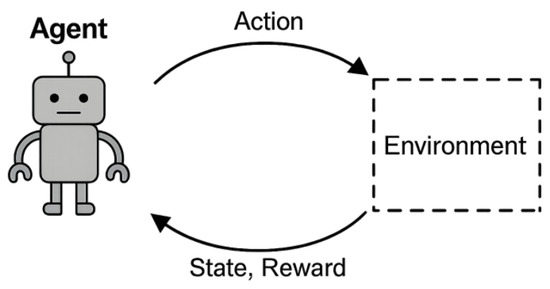
\includegraphics[width=0.4\linewidth]{figures/Single_agent_RL.jpg}
%     \caption{Reinforcement learning agent-environment interaction \cite{ekecki2025uavcontrolsurvey}.}
%     \label{fig:rl_agent}
% \end{figure}

% The policy determines, either stochastically or deterministically, which action the agent should take given a particular \emph{state}. The \emph{state} is a representation of the environment that contains the information needed for decision-making. The \emph{value function} $V(s)$ measures how valuable it is for the agent to be in a given state, based on discounted expected future rewards \cite{brunton2022data}. 

% The objective of RL is to optimize the policy~$\pi$ so as to maximize the expected cumulative future rewards \cite{brunton2022data}.


% \subsubsection{Fundamental RL Concepts}
% Several fundamental concepts are used throughout this thesis and are briefly summarized below.

% \begin{itemize}
%     \item \textbf{Markov Decision Process (MDP)}: Reinforcement learning is commonly
%     formalized as a Markov Decision Process defined by
%     $(\mathcal{S}, \mathcal{A}, P, R, \gamma)$, where an agent in state
%     $s \in \mathcal{S}$ selects an action $a \in \mathcal{A}$, transitions according
%     to $P(s' \mid s,a)$, and receives reward $R(s,a)$. The discount factor
%     $\gamma \in [0,1]$ determines the relative importance of future rewards~\cite{sutton2018rl}.

%     \item \textbf{Exploration vs.\ exploitation}: A central challenge in RL is balancing
%     exploration, where the agent tries new actions to acquire information, and exploitation,
%     where actions believed to yield high return are selected based on current knowledge~\cite{sutton2018rl}.

%     \item \textbf{Reward design and shaping}: Learning is driven by the reward signal.
%     While the task objective may define sparse or terminal rewards, reward shaping can
%     introduce intermediate feedback to accelerate learning. Poorly designed shaping,
%     however, may bias the learned behavior or lead to unintended strategies~\cite{sutton2018rl, brunton2022data}.

%     \item \textbf{Deterministic vs.\ stochastic policies}: Deterministic policies map each state directly to a single action, whereas stochastic policies define a probability distribution over actions. Stochastic policies facilitate exploration and improve robustness under uncertainty and partial observability, while deterministic policies often yield more predictable behavior at execution ~\cite{sutton2018rl, brunton2022data}.

% \end{itemize}


% \subsubsection{RL Methods}
% Reinforcement learning methods can be categorized along several commonly used dichotomies. In this section, the most relevant distinctions for this thesis are briefly introduced ~\cite{sutton2018rl, brunton2022data}.

% \begin{itemize}
%     \item \textbf{Value-based vs.\ policy-based}: Value-based methods learn a value function from which a policy is derived, whereas policy-based methods directly optimize a parameterized policy. Actor-critic methods combine both approaches by learning a policy (actor) guided by a value function (critic).

%     \item \textbf{Model-based vs.\ model-free}: Model-based methods explicitly learn or use a model of the environment dynamics and reward function, while model-free methods learn optimal behavior directly from interaction without estimating the environment model.

%     \item \textbf{Gradient-based vs.\ gradient-free}: Gradient-based methods update policies or value functions using gradient information, whereas gradient-free methods rely on search or evolutionary strategies that do not require differentiable models.

%     \item \textbf{On-policy vs.\ off-policy}: On-policy methods learn from data generated by the current policy, while off-policy methods can learn from data collected using different policies, including past or exploratory behaviors.
% \end{itemize}


% % \subsubsection{Algorithms}
% % Value iteration 
% % Policy itteration
% % Monte carlo learning
% % TD learning
% % Q learning 


% \subsubsection{Deep RL}
% Deep reinforcement learning (DRL) combines reinforcement learning with neural networks (NN) to handle high-dimensional state and action spaces. Neural networks are used as function approximators to represent policies, value functions, or action-value functions, enabling reinforcement learning methods to scale beyond tabular settings \cite{brunton2022data}.

% Typically, these networks consist of multiple layers of interconnected neurons, including one or more hidden layers with non-linear activation functions (e.g. ReLu), which allow the model to capture complex relationships between observations and actions. The network parameters are optimized using gradient-based methods, where learning signals derived from the RL objective are propagated through the network to update the weights \cite{sutton2018rl}.\subsubsection{Algorithms}

% % \subsubsection{Algorithms}
% % Deep policy network 
% % Deep Q learning 


% \subsubsection{Multi-Agent RL (MARL)}

% Multi-Agent Reinforcement Learning (MARL) extends classical reinforcement learning by enabling multiple agents to operate and learn within a shared environment, a setting commonly encountered in coordinated UAV swarm control. Each agent learns a policy while simultaneously influencing, and being influenced by, the actions of other agents, leading to coupled decision-making processes and heterogeneous reward structures. In single-agent reinforcement learning, the environment is typically modeled as a MDP; MARL generalizes this formulation to Markov (stochastic) games, which explicitly capture both environmental dynamics and inter-agent interactions. A graphical representation of this interaction structure is shown in Figure \ref{fig:Multi-Agent Reinforcement Learning 1} \cite{ekecki2025uavcontrolsurvey}.

% \begin{figure}[htbp]
%     \centering
%     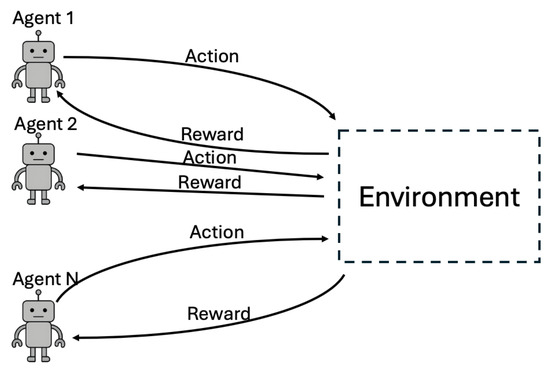
\includegraphics[width=0.4\linewidth]{figures/MARL_picture.jpg}
%     \caption{Graphical representation of Multi-Agent Reinforcement Learning \cite{ekecki2025uavcontrolsurvey}.}
%     \label{fig:Multi-Agent Reinforcement Learning 1}
% \end{figure}

% \paragraph{Challenges in MARL}
% This multi-agent setting introduces several fundamental challenges:

% \begin{itemize}
%     \item \textbf{Credit assignment problem}: Although agents operate within a shared environment and may observe a collective system state, each agent learns its own policy and may receive an individual reward signal. Determining how each agent’s actions contribute to global or collective outcomes is known as the credit assignment problem \cite{sutton2018rl, ekecki2025uavcontrolsurvey}.

%     \item \textbf{Non-stationarity}: From the perspective of any individual agent, the
%     environment becomes non-stationary, as its dynamics continuously change in
%     response to the concurrent learning and actions of other agents \cite{ekecki2025uavcontrolsurvey}.

%     \item \textbf{Curse of dimensionality}: As the number of agents increases, the joint
%     state-action space grows exponentially, leading to high-dimensional representations
%     and significantly increased computational complexity \cite{ekecki2025uavcontrolsurvey, sutton2018rl}.
    
% \end{itemize}

% \paragraph{Learning Paradigms MARL}
% There are several learning paradigms in multi-agent reinforcement learning (MARL) \cite{ekecki2025uavcontrolsurvey}:

% \begin{itemize}
%     \item \textbf{Centralized Learning with Centralized Execution (CLCE):} A single centralized learner optimizes a joint policy using global state and action information and directly controls all agents during execution. While this paradigm simplifies coordination and credit assignment, it scales poorly with the number of agents and relies on continuous availability of global information and centralized control, making it impractical for large-scale or distributed systems.

%     \item \textbf{Decentralized Learning with Decentralized Execution (DLDE):} Each agent independently learns its own policy using only local observations and rewards, and executes actions without centralized coordination. This paradigm is highly scalable and naturally suited to distributed environments; however, it suffers from non-stationarity due to concurrently learning agents and typically struggles to achieve coordinated behavior in cooperative tasks. In addition, because agents are trained without access to global state or other agents’ actions, DLDE is particularly sensitive to partial observability, as the environment appears non-Markovian from an individual agent’s perspective, leading to ambiguous credit assignment and unstable learning dynamics.

%     \item \textbf{Centralized Training with Decentralized Execution (CTDE):} Each agent maintains a decentralized actor network that operates on local observations, while a centralized critic has access to global state information during training. This structure mitigates non-stationarity and enables effective coordination, while preserving decentralized execution at deployment.
    
% \end{itemize}















\chapter{Multi-Agent Reinforcement Learning} \label{app:AppA}

Multi-agent reinforcement learning (MARL) builds upon classical reinforcement learning (RL) methods by considering settings in which multiple agents learn and act simultaneously within a shared environment. However, extending RL techniques to multi-agent systems introduces additional challenges such as non-stationarity, coordination, and scalability, which significantly affect learning stability and performance. RL methods can be broadly divided into two main categories: model-based and model-free approaches. Deep reinforcement learning (DRL) combines RL with deep neural networks to enable learning in high-dimensional state and action spaces. An overview of these approaches is shown in the figure below \cite{brunton2022data}.

\begin{figure}[htbp]
    \centering
    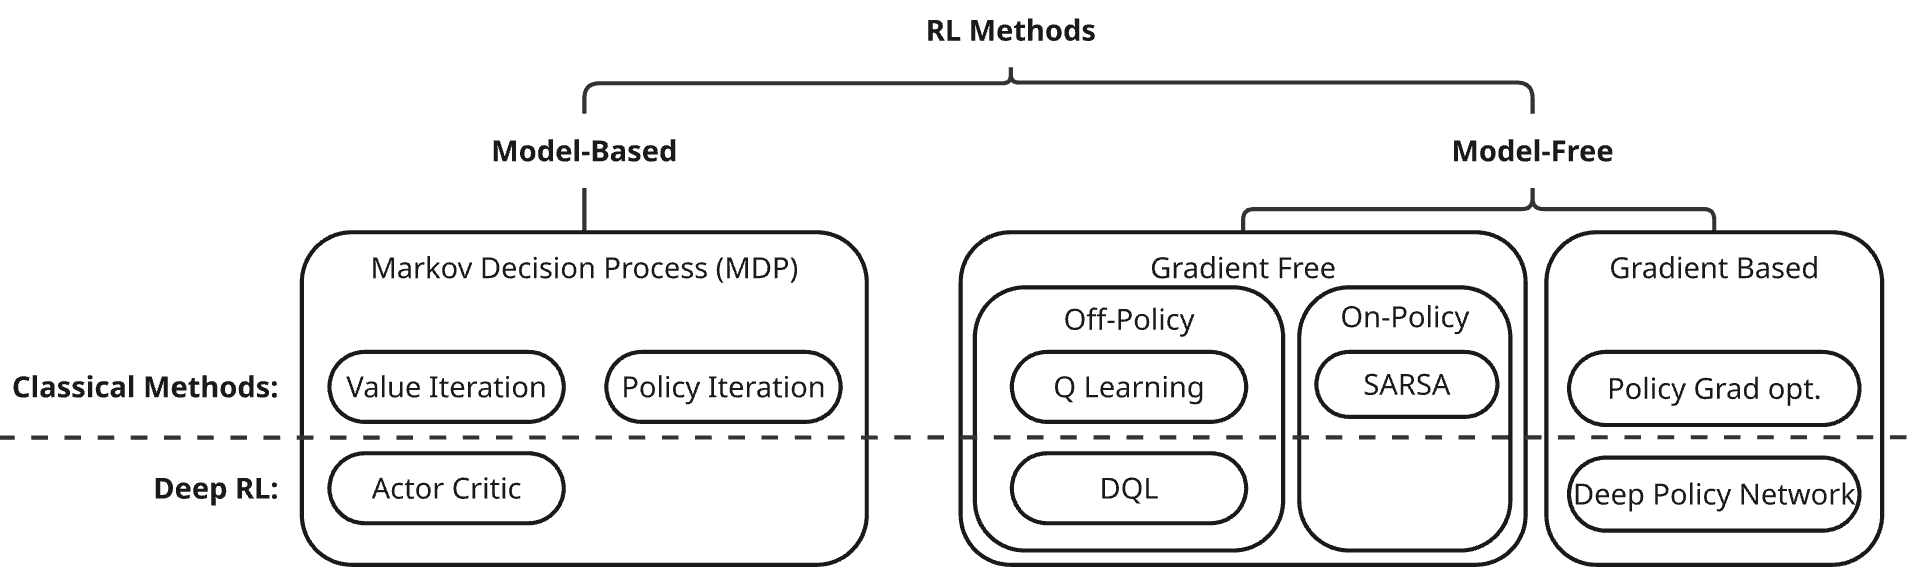
\includegraphics[width=0.9\linewidth]{figures/RL_methods_overview.png}
    \caption{TBU: Overview of RL methods. Adapted from \cite{brunton2022data}.}
    \label{fig:rl_overview}
\end{figure}


\section{Reinforcement Learning}

The basic RL problem consists of several components. An \emph{agent} operates in an \emph{environment}, where it can take \emph{actions} that influence the state of the environment. The agent selects actions according to a \emph{policy}~$\pi$, which can be described by the policy function: \[\pi(s, a) = \Pr(a \mid s).\]

The policy determines, either stochastically or deterministically, which action the agent should take given a particular \emph{state}. The \emph{state} is a representation of the environment that contains the information needed for decision-making. The \emph{value function} V(s) measures how valuable it is for the agent to be in a given state, based on the expected future rewards:

\[
V(s) = \max_{\pi} \; \mathbb{E}_\pi \left[ \sum_{k=0}^{\infty} \gamma^k r_k \,\middle|\, s_0 = s \right].
\]


\begin{figure}[htbp]
    \centering
    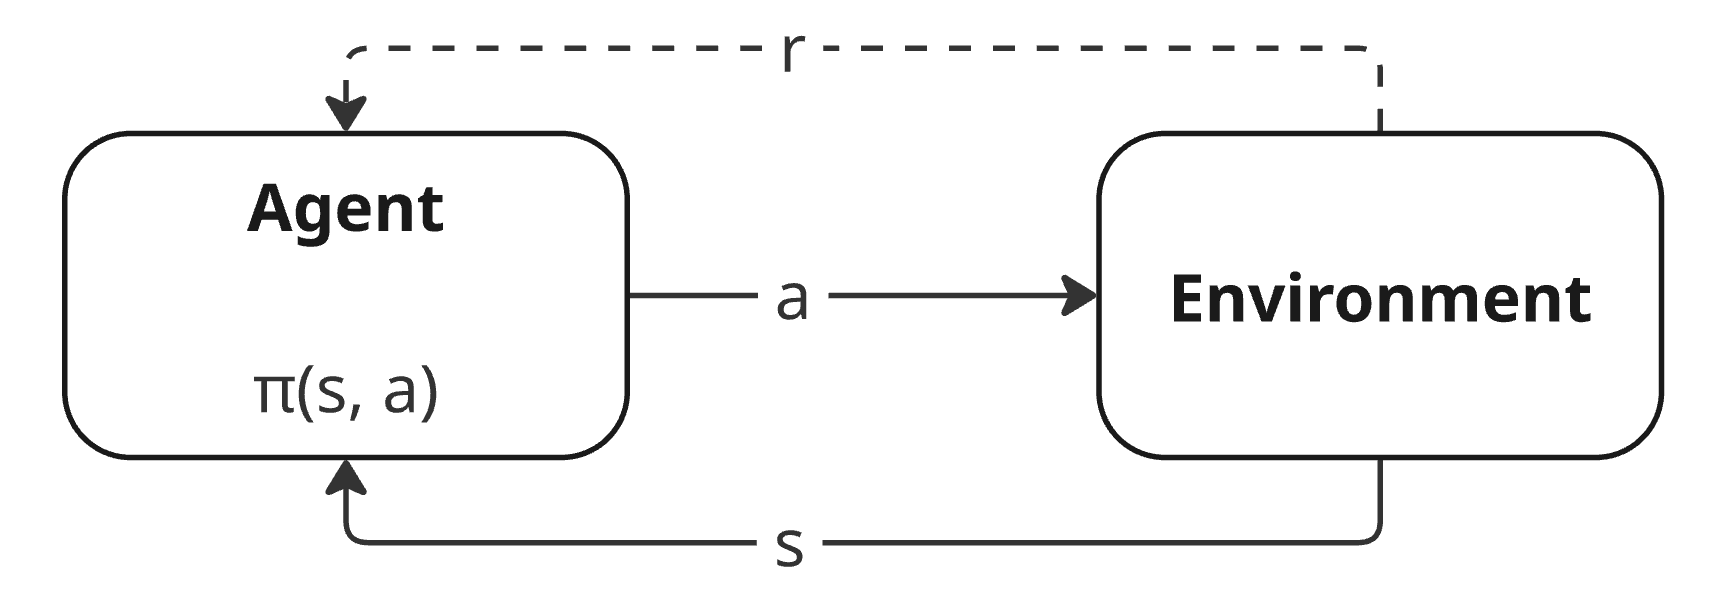
\includegraphics[width=0.5\linewidth]{figures/RL_agent.png}
    \caption{RL agent and environment interactions.}
    \label{fig:rl_overview}
\end{figure}


The objective of RL is to optimize the policy~$\pi$ so as to maximize the expected cumulative future rewards. In MARL multiple agents operate in a shared environment \cite{brunton2022data}.

In RL several key concepts are important to understand: 

\subsection{Model-Based}
Model-based RL can be applied when a sufficiently accurate representation of the environment is available. If the environment is modeled as a \emph{Markov Decision Process} (MDP) with known transition dynamics and reward function methods such as \emph{policy iteration} and \emph{value iteration} can be used. These techniques rely on dynamic programming and the Bellman optimality principle to optimize policies.

Bellman’s equation states that the value function of the current state \(s\) can be expressed recursively as the expected immediate reward plus the discounted value function of the next state:
\[
V(s) = \max_{\pi} \; \mathbb{E}\big[ r_0 + \gamma V(s')]. 
\]

This recursive formulation allows the original problem to be decomposed into smaller subproblems. By repeatedly applying this decomposition, the optimal value function \(V^*(s)\) can be computed. Once the optimal value function is known, an optimal policy can be derived by selecting the action that maximizes the expected return:
\[
\pi^*(s) = \arg\max_{\pi} \; \mathbb{E}\big[ r_0 + \gamma V^*(s') \big].
\]

The main drawback of dynamic programming methods is that they do not scale well to high-dimensional systems, making the computation of optimal policies intractable. In particular, computing the optimal value function requires solving all subproblems over the state and action spaces; when these spaces are large, the number of required computations becomes infeasible. Another limitation is that obtaining an accurate model of the environment or opponents is often infeasible due to unknown dynamics or complex interactions that are difficult to capture \cite{brunton2022data}.

\subsubsection{Value Iteration}
Value iteration is a model-based reinforcement learning method that relies on dynamic programming and Bellman’s optimality equation:
\[
V(s) = \max_{a} \sum_{s'} P(s' \mid s, a)\big( R(s', s, a) + \gamma V(s') \big).
\]

There are two main assumptions. First, a world model \(P\) is available, so the transition to the next state \(s'\) is known for a given state and action. Second, an estimate of the value of the next state \(V(s')\) is maintained through the current value function. The value function is initialized arbitrarily over all states and iteratively updated using the reward function and transition model by maximizing over actions. This process is repeated for all states until the value function converges within a specified tolerance, after which the optimal policy can be extracted~\cite{brunton2022data}.
\[
\pi^*(s) = \arg\max_{a} \sum_{s'} P(s' \mid s, a)
\big( R(s', s, a) + \gamma V^*(s') \big).
\]

\subsubsection{Policy Iteration}
Policy iteration is a model-based method that alternates between two steps: policy evaluation and policy improvement. First, a policy \(\pi\) is initialized (e.g., randomly), and the corresponding value function is computed by iterating the Bellman expectation equation:
\[
V_{\pi}(s) = \mathbb{E}\big[ R(s', s, \pi(s)) + \gamma V_{\pi}(s') \big].
\]

Once the value function has converged, it is held fixed and the policy is improved by sweeping over all actions and selecting the action that maximizes the expected return:
\[
\pi(s) = \arg\max_{a} \; \mathbb{E}\big[ R(s', s, a) + \gamma V_{\pi}(s') \big].
\]

The updated policy is then fixed and the value function is recomputed. This alternating process is repeated until convergence, and policy iteration typically converges in fewer iterations than value iteration~\cite{brunton2022data}.


\subsubsection{Quality Function}
In policy and value iteration, a model of the environment dynamics is required to predict the next state \(s'\) during dynamic programming updates. Introducing a \emph{quality function} (or action-value function) shifts the focus from state values to state-action pairs by directly evaluating the expected return of taking action \(a\) in state \(s\).

The quality function is defined as
\[
\begin{aligned}
Q(s, a)
&= \mathbb{E}\big[ R(s', s, a) + \gamma V(s') \big] \\
&= \sum_{s'} P(s' \mid s, a)\,\bigl(R(s', s, a) + \gamma V(s')\bigr).
\end{aligned}
\]


Through this expectation, the quality function implicitly captures the value of future states. However, this formulation still assumes knowledge of the dynamics of the environment (P) and the reward structure (R). In many real-world problems, these quantities are unknown or difficult to model explicitly.

Once the optimal quality function \( Q^\ast(s,a) \) is obtained, the optimal value function and the corresponding optimal policy can be recovered as~\cite{brunton2022data}

\[
\begin{array}{cc}
V(s) = \max_{a} Q(s,a), & \pi(s) = \arg\max_{a} Q(s,a).
\end{array}
\]



\subsection{Model-Free}
Model-free reinforcement learning does not require an explicit model of the environment dynamics, such as the state transition probabilities, nor does it rely on an explicit representation of the reward structure. Instead, the agent learns directly from interaction with the environment through trial and error. These methods typically scale better to high-dimensional problems, but often require large amounts of data. Model-free approaches can be broadly divided into \emph{gradient-free} and \emph{gradient-based} methods~\cite{brunton2022data}.


\subsubsection{Gradient-Free}
Gradient-free methods estimate value functions or action values without explicitly computing policy gradients. A policy gradient is the gradient of the expected return with respect to the policy parameters. These methods are generally simpler and more stable but can be sample inefficient \cite{brunton2022data}.


\paragraph{Off-Policy}
Off-policy methods learn a target policy while following a different behavior policy, allowing the use of suboptimal or exploratory actions. A key example is \emph{Q-learning}. These methods are data-efficient and enable experience replay, but may suffer from instability when combined with function approximation \cite{brunton2022data}.


\paragraph{Monte Carlo Learning}
Monte Carlo learning is one of the simplest approaches to model-free reinforcement learning. It is applicable to episodic tasks, where each episode has a well-defined terminal state (e.g. end of a game win/loss). In this setting, learning is based on complete episodes, and the return is computed as the cumulative discounted reward over all time steps within an episode. Value estimates are updated only after the episode terminates, using sample averages of observed returns. While Monte Carlo methods are unbiased, they can exhibit high variance and are therefore often inefficient for long-horizon problems \cite{brunton2022data}.

\paragraph{Temporal Difference Learning TD(0)}
Temporal Difference (TD) learning updates value estimates by combining ideas from Monte Carlo methods and ''approximate'' dynamic programming. Instead of waiting until the end of an episode, TD learning updates the value function incrementally at each time step using observed rewards and an estimate of future value.

The value function satisfies the Bellman expectation equation
\[
V(s_k) = \mathbb{E}\bigl[r_k + \gamma V(s_{k+1})\bigr],
\]
which relates the value of a state to the immediate reward and the discounted value of the subsequent state. In model-free reinforcement learning, this expectation is not computed explicitly but is instead approximated using sampled transitions obtained through interaction with the environment.

In TD(0), the value estimate is updated incrementally at each time step according to
\[
V^{\text{new}}(s_k)
= V^{\text{old}}(s_k)
+ \alpha \Bigl(
\underbrace{r_k + \gamma V^{\text{old}}(s_{k+1})}_{\text{TD target estimate}}
-
\underbrace{V^{\text{old}}(s_k)}_{\text{current estimate}}
\Bigr)
\]
\[
\qquad\qquad\;\; = V^{\text{old}}(s_k) + \alpha \,\underbrace{\delta_k}_{\text{TD error}}
\]

where \( \alpha \in (0,1] \) is the learning rate. The temporal difference (TD) error quantifies the difference between the current value estimate \( V^{\text{old}}(s_k) \) and a one-step-ahead approximation \( r_k + \gamma V^{\text{old}}(s_{k+1}) \), referred to as the TD target. This target serves as a sample-based approximation of the Bellman equation and drives learning by adjusting the value estimate toward more accurate predictions of future returns.

TD methods can be extended to \emph{TD(\(n\))} methods by recursively expanding the Bellman equation and the corresponding learning update. This results in value updates that incorporate rewards observed over multiple future time steps. In the limit \( n \to \infty \), TD(\(n\)) converges to Monte Carlo learning. 

TD methods introduce bias but significantly reduce variance compared to Monte Carlo methods. As a result, TD learning is generally more sample-efficient and better suited for long-horizon or continuing tasks~\cite{brunton2022data}.

\paragraph{Q-Learning}
Q-learning is a temporal difference (TD) learning method applied to the action-value function \( Q(s,a) \). Rather than evaluating states alone, Q-learning learns the expected return of taking a specific action \( a \) in a given state \( s \) and thereafter following the optimal policy. Learning occurs through trial-and-error interaction with the environment, without requiring a model of the system dynamics.

The Q-learning update rule is given by
\[
Q^{\text{new}}(s_k,a_k)
=
Q^{\text{old}}(s_k,a_k)
+
\alpha \Bigl(
\underbrace{r_k + \gamma \max_{a} Q^{\text{old}}(s_{k+1},a)}_{\text{TD target}}
-
\underbrace{Q^{\text{old}}(s_k,a_k)}_{\text{current estimate}}
\Bigr),
\]
where \( \alpha \in (0,1] \) is the learning rate. The term in parentheses is the TD error, which measures how different the current estimate is from a one-step-ahead approximation of the optimal action-value function.

Intuitively, if the TD error is negative, the observed reward and future value are lower than expected, and the Q-value for the state--action pair \( (s_k,a_k) \) is decreased. Conversely, a positive TD error indicates that the outcome was better than expected, and the Q-value is increased accordingly. Through repeated updates, Q-values converge toward accurate estimates of long-term returns.

A key feature of Q-learning is the maximization over actions in the TD target. This maximization does not require the agent to follow the current greedy policy during data collection. As a result, the agent may take exploratory or suboptimal actions while still learning the optimal policy. For this reason, Q-learning is classified as an off-policy learning method. Q-learning has faster convergence and higher variance then on-policy methods. Q-learning also enables to learn from imitation and experience replay \cite{brunton2022data}. 

Once the Q-values have converged to their optimal values, the optimal policy can be extracted as
\[
\pi^\ast(s) = \arg\max_{a} Q^\ast(s,a).
\]


\paragraph{On-Policy}
On-policy methods learn the policy that is used to generate data. Exploration is performed by executing the current policy with stochasticity. An example is \emph{SARSA}. These methods are typically more stable but less data-efficient than off-policy approaches \cite{brunton2022data}.

\paragraph{SARSA}
SARSA is an on-policy temporal difference learning algorithm that updates the action-value function using the action actually taken by the current policy. Unlike Q-learning, which maximizes over all possible actions in the update, SARSA uses the next state-action pair \( (s_{k+1}, a_{k+1}) \) generated by the policy itself. As a result, SARSA learns the action-value function corresponding to the behavior policy and is sensitive to the agent’s exploration strategy \cite{brunton2022data}.


\subsubsection{Gradient-Based}
Gradient-based methods, such as \emph{policy gradient} algorithms, directly optimize the policy by following the gradient of the expected return. They are well-suited for continuous action spaces but can suffer from high variance and sensitivity to hyperparameters \cite{brunton2022data}.

\paragraph{Neural Network}



\subsection{Deep Reinforcement Learning}

Deep reinforcement learning (DRL) combines reinforcement learning with neural networks to handle high-dimensional state and action spaces. Neural networks are used as function approximators to represent policies, value functions, or action-value functions, enabling reinforcement learning methods to scale beyond tabular settings.

\paragraph{Deep Policy Network}
The simplest form of DRL is a deep policy network. In this approach, an agent interacts with the environment in the same manner as in classical reinforcement learning, but the state information is provided as input to a neural network. The network outputs either a probability distribution over actions or a deterministic action, thereby defining a policy \( \pi_\theta(a \mid s) \) parameterized by the network weights \( \theta \).

The policy is learned by optimizing the parameters \( \theta \) to maximize the expected cumulative future reward. This is typically achieved using gradient-based optimization, where gradients of a suitable objective function are computed and propagated backward through the network via backpropagation. While the specific network architectures and input representations may vary, all deep policy networks share the common principle of learning policy parameters directly from data using gradient-based methods. Gradient based methods converge much faster then non-gradient based methods like Q-learning \cite{brunton2022data}.

\paragraph{Deep Q-Learning}
Q-learning is an off-policy temporal difference algorithm that learns the optimal action-value function. In Deep Q-Learning (DQL), the Q-function is approximated using a neural network, allowing the method to scale to large or high-dimensional state spaces. Specifically, the action-value function is parameterized as
\[
Q(s,a) \approx Q(s,a;\theta),
\]
where \( \theta \) denotes the network parameters.

This approximation is essential when the state–action space is prohibitively large, making tabular methods infeasible. By leveraging the generalization capability of neural networks, DQL can learn meaningful representations of the state space and estimate Q-values efficiently.

Learning is performed by minimizing a squared temporal difference error, given by the loss function
\[
\mathcal{L}(\theta)
=
\mathbb{E}\Bigl[
\bigl(
r_k + \gamma \max_a Q(s_{k+1},a;\theta)
-
Q(s_k,a_k;\theta)
\bigr)^2
\Bigr].
\]
The network parameters \( \theta \) are optimized using stochastic gradient descent and backpropagation, driving the Q-function toward consistency with the Bellman optimality equation \cite{brunton2022data}.


\paragraph{Actor-Critic Networks}
Actor-critic methods combine ideas from both policy-based and value-based reinforcement learning. In this framework, two function approximators are learned simultaneously:

\begin{itemize}
    \item \textbf{Actor:} The actor learns a parameterized policy which determines the action selection given a state.
    \item \textbf{Critic:} The critic evaluates the actor’s policy by learning a value function, such as the state-value function or the action-value function \( Q_w(s,a) \), parameterized by weights \( w \).
\end{itemize}

The critic provides a learning signal that evaluates the quality of the actor’s actions, typically through a temporal difference error or an advantage estimate. A common example of this approach is the Advantage Actor--Critic (A2C) method, in which the actor is updated using advantage estimates to reduce variance and improve learning stability. This approach differs fundamentally from Q-learning, which relies solely on value-based optimization and derives the policy only after learning the action-value function \cite{brunton2022data}.


% \subsection{Method Summary}
% TBD



\section{Multi-Agent Reinforcement Learning}

Multi-Agent Reinforcement Learning (MARL) extends classical reinforcement learning by enabling multiple agents to operate and learn within a shared environment, a setting commonly encountered in coordinated UAV swarm control. Each agent learns an individual policy while simultaneously influencing, and being influenced by, the actions of other agents, leading to coupled decision-making processes and heterogeneous reward structures. In single-agent reinforcement learning, the environment is typically modeled as a Markov Decision Process (MDP); MARL generalizes this formulation to Markov (stochastic) games, which explicitly capture both environmental dynamics and inter-agent interactions. A graphical representation of this interaction structure is shown in Fig.~\ref{fig:Multi-Agent Reinforcement Learning} \cite{ekecki2025uavcontrolsurvey}.

\begin{figure}[htbp]
    \centering
    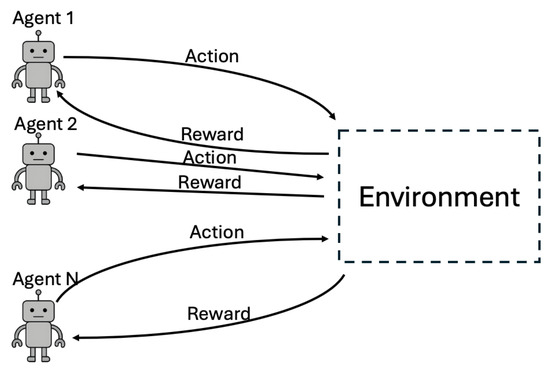
\includegraphics[width=0.4\linewidth]{figures/MARL_picture.jpg}
    \caption{Graphical representation of Multi-Agent Reinforcement Learning. Adapted from \cite{ekecki2025uavcontrolsurvey}.}
    \label{fig:Multi-Agent Reinforcement Learning}
\end{figure}

This setting introduces several fundamental challenges. Although agents operate within a single shared environment and observe a collective system state, each agent must learn its own policy and may receive distinct rewards. Furthermore, from the perspective of any individual agent, the environment becomes non-stationary, as its dynamics evolve in response to the concurrent learning and actions of other agents. As the number of agents increases, the joint state–action space grows exponentially, leading to high-dimensional system representations and the well-known curse of dimensionality, which significantly increases computational complexity.

MARL algorithms are commonly categorized into value-based, policy-based, and actor–critic approaches. Among these, actor–critic methods are widely adopted due to their ability to combine stable value estimation with efficient policy optimization, making them particularly well suited for high-dimensional and continuous control tasks \cite{ekecki2025uavcontrolsurvey}.


\subsection{Value-Based Methods}
The primary objective of value-based reinforcement learning methods is to estimate the optimal state–action value function, commonly referred to as the Q-function. A policy is derived by selecting actions greedily with respect to the estimated Q-function, which inherently restricts these methods to discrete action spaces. In UAV applications, this limitation can be mitigated by discretizing the environment, for example through the use of grid-world representations for tasks such as area coverage. In such scenarios, a UAV’s action set is limited to a finite number of movements, such as moving left, right, or forward within the grid. Consequently, value-based MARL methods operate in discrete action spaces and are well suited for structured missions that can be naturally discretized \cite{ekecki2025uavcontrolsurvey}.

\paragraph{QMIX}
QMIX is a multi-agent reinforcement learning algorithm that enables decentralized execution through centralized training. During training, each agent learns a local action–value function based on its own partial observations, while a centralized mixing network combines these individual Q-functions using global state information. The mixing network is constrained to be monotonic, ensuring that locally greedy action selections are consistent with maximizing the global joint action–value function. While this design allows QMIX to scale efficiently and operate under partial observability, it limits the algorithm’s ability to represent non-monotonic value functions, making it less suitable for tasks that require highly coordinated or complex joint behaviors \cite{ekecki2025uavcontrolsurvey}.

\begin{figure}[htbp]
    \centering
    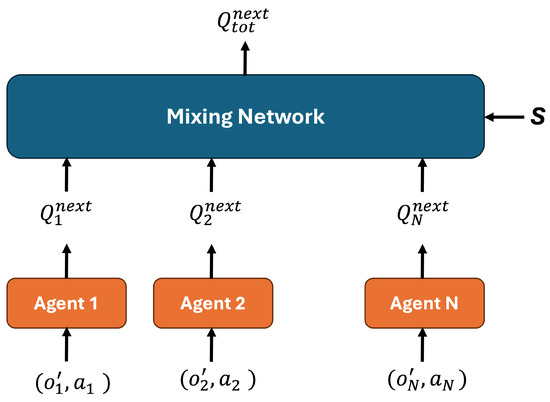
\includegraphics[width=0.4\linewidth]{figures/Qmix.jpg}
    \caption{Graphical representation of QMIX. Adapted from \cite{ekecki2025uavcontrolsurvey}.}
    \label{fig:QMIX}
\end{figure}



\paragraph{Deep Q-Network (DQN)}
In multi-agent Deep Q-Network (DQN) approaches, each agent independently applies the principles of deep Q-learning, using neural networks as function approximators for the Q-function. To improve training stability, DQN employs experience replay and a target network. In this decentralized setting, agents learn and execute their policies independently, without explicit coordination or information sharing during training or execution. While this simplicity enables straightforward implementation, it can lead to non-stationarity and suboptimal coordination in multi-agent environments \cite{ekecki2025uavcontrolsurvey}.

\begin{figure}[htbp]
    \centering
    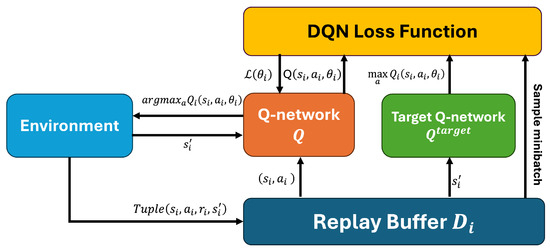
\includegraphics[width=0.4\linewidth]{figures/DeepQNetwork.jpg}
    \caption{Graphical representation of Deep Q-Network (DQN). Adapted from \cite{ekecki2025uavcontrolsurvey}.}
    \label{fig:Deep Q-Network (DQN)}
\end{figure}


\begin{table}[htbp]
\centering
\caption{Comparison of QMIX and Multi-Agent DQN. Adapted from \cite{ekecki2025uavcontrolsurvey}.}
\label{tab:qmix_dqn_comparison}
\begin{tabular}{lcc}
\hline
\textbf{Feature} & \textbf{QMIX} & \textbf{DQN} \\
\hline
Partial observability & Supported & Limited \\
Scalability & High & Moderate \\
Centralized training & Yes & No \\
Decentralized execution & Yes & Yes \\
\hline
\end{tabular}
\end{table}


\subsection{Policy-Based Methods}
Policy-based reinforcement learning methods directly optimize the agents’ policies, in contrast to value-based approaches that first learn a value function and subsequently derive a policy from it. By optimizing the policy parameters explicitly, these methods are well suited for high-dimensional and continuous action spaces. 

Actor–critic methods represent a prominent subclass of policy-based approaches, combining the advantages of both value-based and policy-based learning. This combination improves learning stability and sample efficiency, particularly in partially observable, complex, and dynamic environments.

Despite these advantages, policy-based MARL methods face several challenges, most notably non-stationarity arising from the simultaneous learning of multiple agents. Centralized Training with Decentralized Execution (CTDE) has been widely adopted to mitigate this issue. Additional challenges include scalability, efficient inter-agent communication, and robustness under partial observability \cite{ekecki2025uavcontrolsurvey}.


\paragraph{Deep Deterministic Policy Gradient (DDPG)}
Deep Deterministic Policy Gradient (DDPG) is an actor–critic, model-free reinforcement learning method that employs a deterministic policy and is well suited for continuous action spaces. In multi-agent settings, DDPG is commonly applied within a centralized training and decentralized execution (CTDE) framework. During training, each agent maintains its own critic network, which has access to global state information and the actions of all agents, while each agent learns an individual actor network. 

This architecture introduces scalability challenges, as the number of critic networks grows linearly with the number of agents. Furthermore, the assumption that critics have access to full state information may limit applicability in partially observable environments. Despite these limitations, DDPG and its multi-agent variants have demonstrated strong performance in cooperative multi-robot and multi-UAV tasks, where agents are able to learn coordinated behaviors and effective joint strategies \cite{ekecki2025uavcontrolsurvey}.

\begin{figure}[htbp]
    \centering
    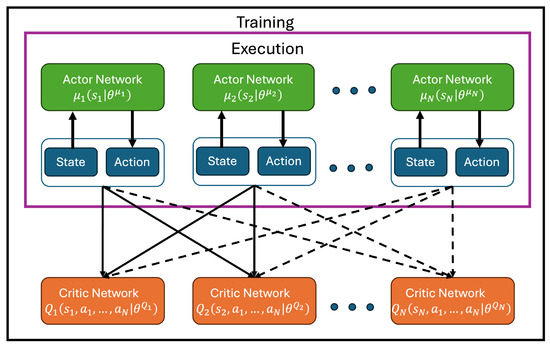
\includegraphics[width=0.4\linewidth]{figures/DDPG.jpg}
    \caption{Graphical representation of Deep Deterministic Policy Gradient. Adapted from \cite{ekecki2025uavcontrolsurvey}.}
    \label{fig:Deep Deterministic Policy Gradient}
\end{figure}

\paragraph{Trust Region Policy Optimization (TRPO)}
Trust Region Policy Optimization (TRPO) is a policy-based reinforcement learning method designed to ensure stable policy updates by constraining the change between successive policies. This is achieved by enforcing a trust region through a Kullback–Leibler (KL) divergence constraint, which prevents excessively large policy updates that could degrade performance. In multi-agent settings, TRPO enables agents to optimize their policies based on local observations and individual rewards, while training is commonly performed under centralized training and decentralized execution (CTDE). 

Multi-agent TRPO is particularly effective in environments that require decentralized coordination under partial observability, communication constraints, or limited reliance on GPS. These characteristics make it well suited for complex and adversarial domains, such as military applications.

An extension of this approach is heterogeneous-agent TRPO, which employs sequential policy optimization to enable agents with different roles or capabilities to learn distinct policies within a shared environment \cite{ekecki2025uavcontrolsurvey}.

\begin{figure}[htbp]
    \centering
    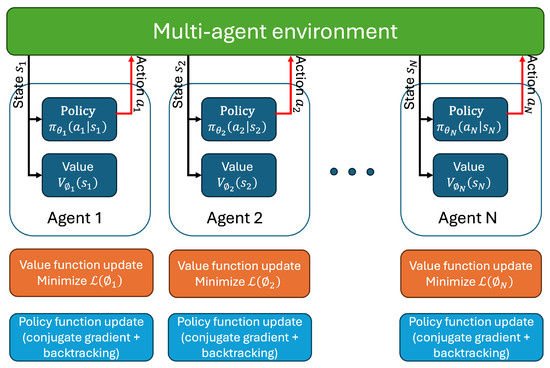
\includegraphics[width=0.4\linewidth]{figures/TRPO.jpg}
    \caption{Graphical representation of MATRPO. Adapted from \cite{ekecki2025uavcontrolsurvey}.}
    \label{fig:TRPO}
\end{figure}


\paragraph{Proximal Policy Optimization (PPO)}
Proximal Policy Optimization (PPO) builds upon Trust Region Policy Optimization (TRPO) by providing a simpler and more computationally efficient method for stabilizing policy updates. Instead of enforcing a hard trust-region constraint through a Kullback–Leibler (KL) divergence penalty, PPO regulates policy updates by balancing the deviation between the current policy and the previous policy, thereby preventing excessively large parameter updates.

PPO is typically trained using batches of collected trajectory data, which are processed through mini-batch stochastic gradient descent. In this context, batching refers to collecting multiple state–action–reward trajectories before updating the policy, while mini-batch gradient descent updates the network parameters using smaller subsets of this data. This approach improves sample efficiency and training stability.

In multi-agent settings, PPO is commonly applied within a centralized training and decentralized execution (CTDE) framework. Each agent maintains a decentralized actor network that operates on local observations, while a centralized critic has access to global state information during training. This structure mitigates non-stationarity and enables effective coordination, while preserving decentralized execution at deployment \cite{ekecki2025uavcontrolsurvey}.


\begin{figure}[htbp]
    \centering
    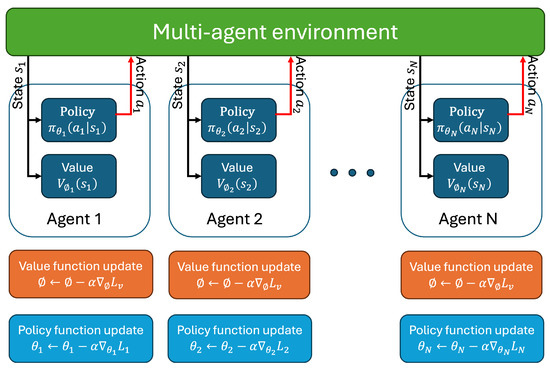
\includegraphics[width=0.4\linewidth]{figures/PPO.jpg}
    \caption{Graphical representation of PPO. Adapted from \cite{ekecki2025uavcontrolsurvey}.}
    \label{fig:PPO}
\end{figure}

A comparison between policy based methods is provided in table \ref{tab:marl_comparison_hml}. Although PPO demonstrates strong stability and scalability, its on-policy nature and conservative update mechanism can limit sample efficiency and fine-grained coordination, making alternative MARL approaches more suitable for precision-critical or tightly coupled multi-agent control tasks \cite{ekecki2025uavcontrolsurvey}.

\begin{table}[htbp]
\centering
\caption{Qualitative Comparison of MADDPG, TRPO, and PPO. Adapted from \cite{ekecki2025uavcontrolsurvey}.}
\label{tab:marl_comparison_hml}
\begin{tabular}{lccc}
\hline
\textbf{Criterion} & \textbf{MADDPG} & \textbf{TRPO} & \textbf{PPO} \\
\hline
Action space  & Continuous & Continuous & Discrete and Continuous \\
Policy  & Deterministic & Stochastic & Stochastic \\
Training stability & Medium & Medium & High \\
Scalability to many agents & Medium & Low & High \\
Use in MARL research & High & Low & High \\
Computational efficiency & Medium & Low & High \\
Convergence speed & Low & Medium & High \\
Convergence accuracy & Medium & Medium & High \\
Implementation simplicity & Medium & Low & High \\
\hline
\end{tabular}
\end{table}


\subsection{Federated Learning Methods}
Federated learning (FL)–based multi-agent reinforcement learning enables agents to collect experiences, state observations, and rewards locally, thereby supporting fully distributed control. In this framework, each agent trains its own local model, and the learned parameters are periodically aggregated by a central server using methods such as Federated Averaging. Unlike centralized or CTDE approaches, federated MARL does not require access to global state information, making it particularly suitable for environments where global observability is limited or unavailable.

Federated learning is especially advantageous in scenarios with strict data privacy requirements, limited communication bandwidth, or intermittent connectivity. By sharing model parameters instead of raw experience data, FL reduces communication and preserves local data confidentiality, while still enabling coordinated learning across agents \cite{ekecki2025uavcontrolsurvey}.


\subsection{Summary: Method Comparison}
To assess which learning paradigm is most suitable for the considered application, a comparative summary adapted from \cite{ekecki2025uavcontrolsurvey} is provided below. 

Value-based MARL methods focus on learning value functions and are best suited for relatively simple, discrete environments with limited action spaces. These methods are generally easier to implement and interpret; however, they often suffer from scalability issues as the state space grows and can become unstable in partially observable environments.

Policy-based MARL methods directly optimize centralized or decentralized policies, frequently combining policy learning with value estimation in actor–critic architectures and adopting a centralized training and decentralized execution (CTDE) paradigm. These methods exhibit greater adaptability to continuous control tasks and dynamic environments. While they typically require more training samples and may converge more slowly, the resulting policies are generally more robust and flexible in complex multi-agent scenarios.

Federated MARL enables distributed policy learning by allowing agents to train locally while sharing only model parameters, rather than raw state or experience data. This approach offers strong privacy preservation and high scalability, making it particularly suitable for large-scale, communication-constrained, or privacy-sensitive multi-agent systems.


\begin{table}[htbp]
\centering
\caption{Comparison of MARL Paradigms. Adapted from \cite{ekecki2025uavcontrolsurvey}.}
\label{tab:marl_paradigms_short}
\begin{tabular}{lccc}
\hline
\textbf{Criterion} & \textbf{Value-Based} & \textbf{Policy-Based} & \textbf{Federated MARL} \\
\hline
Learning objective & Value functions & Policies & Distributed policies \\
Action space & Discrete & Discrete / Continuous & Discrete / Continuous \\
Best use case & Structured cooperation & Continuous control & Distributed systems \\
Observability & Full / Low-noise & Partial / Dynamic & Local only \\
Scalability & Medium & High & High \\
Communication cost & Low–Medium & Medium & Low \\
Training stability & Medium & High & Medium \\
Adaptability to dynamic environments & Low–Medium & High & High \\
Privacy preservation & No & No & Yes \\
Best UAV suitability & Discrete tasks & Continues control & Privacy-constrained  \\
\hline
\end{tabular}
\end{table}




% 

\chapter{Existing Research}

This chapter provides an overview of existing research on combat unmanned aerial vehicles (UAVs), with a particular focus on strike and electronic warfare (EW) missions. First, the relevant literature is briefly summarized. Next, the mission types and operational constraints considered in existing studies are reviewed. Subsequently, the control methods proposed in the literature are examined and compared. Finally, this chapter identifies key research gaps and limitations in current work, thereby motivating the research directions pursued in this thesis.


\section{Summery of Literature}
In this section a summery of existing literature is given. First a summery of the scenario is given, followed by the proposed solution method. After a discussion on the proposed scenario and method is provided related to the objectives of this thesis. 

\subsubsection{MADQN and IAPPO for EA and SEAD mission, Yue et al., 2022}
In \cite{yue2022uav_sead_hmarl}, a team of heterogeneous fighter–jammer UAV duos, modeled as kinematic point masses, is tasked with executing a SEAD mission. Each jammer suppresses an IADS to reduce its detection range, enabling the paired fighter to approach and destroy the target. The scenario assumes full observability and unrestricted communication, with all target locations known throughout the mission.

The authors propose a hierarchical MARL framework in which target allocation is solved at a high level using a multi-agent deep Q-network (MADQN), while low-level cooperative control is handled using independent asynchronous proximal policy optimization (IAPPO). Each fighter–jammer duo is controlled by a shared policy with continuous action outputs (velocity and heading for both UAVs). The learning is independent, as each duo optimizes its own policy without a centralized critic, which improves scalability but introduces non-stationarity. Asynchrony is achieved through parallel experience collection and unsynchronized policy updates, improving sample efficiency relative to standard PPO. Target allocation is performed sequentially, with each duo treated as a DQN agent, and exploration is enhanced using a Metropolis criterion \cite{yue2022uav_sead_hmarl}.

Despite demonstrating scalability in simplified scenarios, the proposed approach has several limitations that reduce its applicability to realistic and dynamic environments. The fixed pairing of fighters and jammers under a shared policy constrains adaptability and enforces close-formation behavior tailored to a specific mission structure. As a result, the method does not generalize well to scenarios involving dynamic re-tasking, emerging threats, or alternative team compositions. Furthermore, the independent PPO formulation leads to a non-stationary learning environment, which is likely to become unstable as adversary complexity or agent interactions increase.

The hierarchical structure also enforces a strict allocate-then-execute paradigm, preventing reallocation or mission-level adaptation during execution. These capabilities are essential in contested and uncertain operational settings. Additionally, the method assumes the existence of a central coordinating agent with global communication and perfect information during target allocation, neglecting practical limitations on communication, sensing, and information reliability in SEAD missions. Finally, adversaries are modeled as static, fully known entities, further limiting the realism of the evaluation.

\subsubsection{Centralized PPO in strike mission, Yulsek et al., 2021}
In \cite{yuksek2021cooperative}, a reinforcement learning (RL)–based centralized path-planning method for a fleet of Unmanned Combat Aerial Vehicles (UCAVs) operating in a hostile environment. The goal is for multiple UCAVs to reach a target simultaneously, avoid no-fly zones (NFZs) that represent enemy air defenses. The UCAVs are assumed to operate at constant velocity and control actions are lateral accelerations by a centlised agent. 



\section{Mission types and Operational Constraints}


\begin{table}[htbp]
\centering
\caption{Mapping of operational constraints to mission types addressed in the literature. Empty cells indicate limited or no explicit treatment.}
\label{tab:mission_constraints_empty}
\begin{tabular}{lccc}
\toprule
\textbf{Operational Constraint}
& \textbf{Strike}
& \textbf{EW}
& \textbf{Strike + EW} \\
\midrule
Partial observability 
& \cite{Wang2025CooperativeUAV}
& 
& \\

Communication limitations  
& \cite{Wang2025CooperativeUAV}
& 
& \\

Adversaries / Interceptors (fixed or mobile)
& \cite{Wang2025CooperativeUAV}
& 
& \cite{xu2025mdrl_uav_combat, yue2022uav_sead_hmarl} \\

No-fly-zones 
& \cite{yuksek2021cooperative}
& 
& \\

Temporal and spatial coordination requirements 
& \cite{yuksek2021cooperative}
& 
& \\

Heterogeneous agents (e.g. striker, jammer)
& \cite{Wang2025CooperativeUAV}
& 
& \cite{yue2022uav_sead_hmarl} \\

% GNSS-denied or degraded navigation 
% & 
% & 
% & \\

\bottomrule
\end{tabular}
\end{table}




\section{Overview of MARL Methods}

\begin{table}[htbp]
\centering
\caption{Overview of multi-agent reinforcement learning control methods used in cooperative autonomous systems.}
\label{tab:marl_methods}
\begin{tabular}{llcc}
\toprule
\textbf{Method Class} 
& \textbf{Specific Method} 
& \textbf{Citations} 
& \textbf{Notes} \\
\midrule

\multirow{2}{*}{Value-based}
& MADQL 
& \cite{yue2022uav_sead_hmarl} 
& \cite{yue2022uav_sead_hmarl} uses MADQL for task allocation \\

& QMIX 
& -- 
& notes \\

\midrule
\multirow{2}{*}{Actor--Critic}
& MAPPO 
& \cite{yue2022uav_sead_hmarl}
& \cite{yue2022uav_sead_hmarl} uses IAPPO for continuous motion control \\

& MADDPG 
& -- 
& notes \\

\bottomrule
\end{tabular}
\end{table}


%\input{appendix/task_distribution.tex}
%\input{appendix/appendix-b}
%\input{appendix/appendix-c} % Create file to add

\end{document}
